% CVPR template (https://github.com/cvpr-org/author-kit), camera-ready style with page numbers.
\documentclass[10pt,twocolumn,letterpaper]{article}
\usepackage[pagenumbers]{cvpr}
\usepackage{graphicx,booktabs,amsmath,amssymb,multirow,xcolor}
\usepackage[T1]{fontenc}
\definecolor{cvprblue}{rgb}{0.21,0.49,0.74}
\usepackage[breaklinks,colorlinks,allcolors=cvprblue]{hyperref}
\hypersetup{pdftitle={Three-Class Diabetic Retinopathy Referral Triage with a Sensitivity Guarantee for Each Class},
  pdfauthor={Swayam Sahu, Sahil Sihag, Nitesh Kumar},
  pdfsubject={Machine Learning course project, IIT Jodhpur},
  pdfkeywords={diabetic retinopathy, conformal prediction, referral triage, distribution shift}}
\def\confName{CVPR}
\def\confYear{2027}
\newcommand{\pct}{\,\%}
\setlength{\tabcolsep}{3pt}

\title{Three-Class Diabetic Retinopathy Referral Triage\\with a Sensitivity Guarantee for Each Class}
\author{Swayam Sahu\qquad Sahil Sihag\qquad Nitesh Kumar\\
M.Tech (Data and Computational Sciences), Department of Mathematics, IIT Jodhpur\\
{\tt\small m26mac010@iitj.ac.in \quad m26mac008@iitj.ac.in \quad m24ma2006@iitj.ac.in}\\
{\small Code: \url{https://github.com/Nova1369/dr-referral-triage}}}

\begin{document}
\maketitle

\begin{abstract}
Our referral rule turns one fundus photo into \emph{no referral}, \emph{routine referral} or \emph{urgent referral}, with a stated guarantee for each class. On 3,662 APTOS photos it sends home 4.2\pct{} of referable eyes (95\pct{} CI 3.2--5.2; target ${\le}10$\pct) and refers 91.2\pct{} of urgent eyes urgently (88.3--93.8; target ${\ge}90$\pct); the plain most-likely-class decision reaches only 12.8\pct{} and 46.3\pct. The rule (C1) sets one conformal threshold per class on the probabilities of a logistic regression on frozen ResNet-50 features (referable AUROC 0.973). At a new clinic APTOS thresholds fail (Messidor-2: 80\pct{} of referable eyes sent home); refitting the three thresholds on labelled local photos (C2) restores both targets from about 50 photos at IDRiD and 300 at Messidor-2. The guarantee does not move with prevalence, but the workload does, and it can be forecast from unlabelled photos (C3). Additional work shows that a per-class guarantee is not a per-group one: on mostly-healthy APTOS cameras the model reads the camera, not the retina. Of ten fixes compared with significance tests, six restore every camera group, and our camera-decorrelated weights cost the fewest healthy eyes. A new method, C2-IW, chooses which local photos to label and cuts the labels C2 needs at Messidor-2 by about a third.
\end{abstract}

\section{Introduction}
About 101 million Indian adults have diabetes~\cite{indiab}, and 12.5\pct{} of them have diabetic retinopathy (DR)~\cite{smart}. Graders are scarce, while AI grades DR about as well as experts~\cite{gulshan16,gulshan19}. What screening programmes lack is a referral rule with a \emph{stated} sensitivity that survives a move to a new clinic.

We group the five-grade international scale~\cite{wilkinson} as in the ICO guidelines~\cite{ico}: grades 0--1 \emph{no referral}, grade 2 \emph{routine}, grades 3--4 \emph{urgent}. Targets: at most 10\pct{} of eyes needing referral (grades 2--4) may be sent home, and at least 90\pct{} of grade 3--4 eyes must be referred urgently, at APTOS and, after recalibration, at a new clinic. Eyes the rule cannot decide go to a human grader.

\textbf{Contributions.} (C1) a class-wise (Mondrian) conformal referral rule with a guarantee per class; (C2) its recalibration at a new clinic from $k$ labelled photos; (C3) its behaviour and workload under prevalence shift; experiments E0 (reproducing the coverage drop of standard conformal prediction at new clinics~\cite{hasan}), E1 (eleven course models under nested cross-validation), E2, E3, baselines B0--B9, ablations and an error analysis. Section~\ref{sec:extra}, kept separate, reports work beyond the proposal: does the guarantee hold for every group of patients?

\section{Data and preprocessing}
\begin{table*}[t]\centering\small
\resizebox{\textwidth}{!}{\begin{tabular}{@{}llrlll@{}}\toprule
Dataset & Site and camera & Photos & Grades 0/1/2/3/4 & No ref.\ / routine / urgent & Role\\\midrule
APTOS 2019~\cite{aptos} & Aravind Eye Hospital, India; 17 photo sizes & 3,662 & 1,805/370/999/193/295 & 2,175 (59.4\pct) / 999 (27.3\pct) / 488 (13.3\pct) & training, internal test\\
IDRiD~\cite{idrid} & eye clinic, Nanded, India; one camera & 516 & 168/25/168/93/62 & 193 (37.4\pct) / 168 (32.6\pct) / 155 (30.0\pct) & new clinic 1\\
Messidor-2~\cite{decenciere,abramoff13} & three French hospitals; one camera model & 1,744 & 1,017/270/347/75/35 & 1,287 (73.8\pct) / 347 (19.9\pct) / 110 (6.3\pct) & new clinic 2\\\bottomrule
\end{tabular}}
\caption{Data: 5,922 gradable photos. APTOS test labels were never released, so its 3,662 training photos are used with cross-validation; IDRiD uses its 413 training and 103 test photos; Messidor-2 grades are the adjudicated grades of Krause \etal~\cite{krause} (1,744 gradable of 1,748).}\label{tab:data}
\end{table*}
We use 5,922 gradable photos from three public datasets (Tab.~\ref{tab:data}). APTOS trains and tests the models; IDRiD and Messidor-2 play two new clinics. The Messidor-2 licence forbids redistribution, including processed copies, so no Messidor-2 image appears here or in the repository. Each photo is cropped to a square around its circular retina (RANSAC circle fit, median overlap 0.993--0.997), resized to $512{\times}512$, and the outside is blacked out; colours are not changed. A high-pass signature found 290 copied photos in 141 clusters (40 with conflicting grades). Copies, look-alike pairs and the two eyes of a Messidor-2 exam share a group; APTOS is split into 10 grade-stratified folds with no group split across folds.

\section{Method}
\textbf{Features and models.} Each photo becomes 2,048 numbers from a frozen ImageNet ResNet-50~\cite{he,timm} at 224\,px. Eleven course models are trained on them (logistic regression, naive Bayes, LDA, QDA, $k$-NN, decision tree, random forest, AdaBoost, gradient boosting, SVM, MLP)~\cite{sklearn}. Multinomial L2 logistic regression ranks best (tied with the SVM) and is carried forward.

\textbf{Conformal prediction.} For a calibration photo with class $y$ the score is $s=1-\hat p(y\mid x)$~\cite{sadinle}. From $n$ calibration scores the threshold $\hat q$ is the $\lceil (n+1)(1-\alpha)\rceil$-th smallest, and $C(x)=\{c: 1-\hat p(c\mid x)\le \hat q\}$ covers the true class with probability $\ge 1-\alpha$ under exchangeability~\cite{vovk,ahamed}. Standard conformal prediction (B4) uses one threshold, so its 90\pct{} is an average over classes.

\textbf{C1: one threshold per class.} Mondrian conformal prediction~\cite{vovk} fits $\hat q_c$ on calibration photos of class $c$ only, so $P(c\in C(x)\mid y=c)\ge 1-\alpha$ for each class. A class needs $\ge 1/\alpha-1=9$ calibration photos for a finite threshold. Decision: urgent if \emph{urgent}$\,\in C(x)$; routine if $C(x)=\{\text{routine}\}$; no referral if $C(x)=\{\text{no referral}\}$; otherwise a grader decides. A referable eye is sent home only if its set is exactly \{no referral\}, i.e.\ its class is left out, so 90\pct{} coverage of routine and urgent caps referable eyes sent home at 10\pct; 90\pct{} urgent coverage is the second target. C1 uses raw probabilities: isotonic calibration learnt on APTOS maps 16--17\pct{} of Messidor-2's sick eyes to exactly 0, which ties the scores.

\textbf{C2: a new clinic.} Keep the APTOS model and refit only the three thresholds on $k$ labelled local photos. The rarest class decides how many are needed.

\textbf{C3: prevalence and workload.} Under label shift each class threshold still covers its class~\cite{podkopaev}. With $r_y$ the share of class-$y$ eyes referred, referrals per 1,000 eyes are $1000\sum_y \pi_y r_y$; C3 estimates the clinic's class shares $\pi$ from unlabelled photos by EM~\cite{saerens} and adjusts each eye's risk by $p(y\mid x)\pi_y/\pi^{\text{APTOS}}_y$.

\textbf{Baselines.} B0 refer no one / everyone; B1 class shares; B2 gradient boosting on image quality and photo size only; B3 two tuned thresholds on $P(\text{referable})$ and $P(\text{urgent})$~\cite{gulshan16,abramoff16}; B4 standard conformal~\cite{hasan}; B5 uncertain band (top probability $<0.6$); B6 APTOS thresholds unchanged; B7 retraining on (a) the $k$ local photos, (b) APTOS plus them; B8 workload with APTOS shares; B9 with the true shares (oracle).

\textbf{Protocol.} Every APTOS photo is decided once, by a model and rule that never saw it or a copy. In each of 10 outer folds, 15\pct{} of the training split is held out for calibration (about 495 photos); the rest is split into 5 inner folds for model selection (mean of referable and urgent AUROC). E2: logistic regression ($C{=}0.003$) trained on all APTOS; for each clinic and $k$, 200 draws of $k$ local photos by whole groups, tested on the clinic's other photos. E3: APTOS split by group into halves 200 times; half B is resampled to 5, 12.5 or 25\pct{} referable eyes. Intervals: 1,000 group-bootstrap resamples (shared by all models), Wilson intervals for subgroups. Seed 42 throughout; \texttt{check\_splits.py} confirms no group crosses training, calibration and test sets.

\section{Results}
\subsection{E1 and E0}
\begin{table}[t]\centering\small
\resizebox{\linewidth}{!}{\begin{tabular}{@{}lccc@{}}\toprule
Model & AUROC referable & AUROC urgent & QWK\\\midrule
Logistic regression & \textbf{0.973} (0.968--0.977) & \textbf{0.920} & 0.766\\
SVM (RBF) & \textbf{0.973} (0.968--0.977) & 0.919 & 0.766\\
LDA & 0.964 (0.958--0.969) & 0.913 & 0.772\\
MLP & 0.963 (0.957--0.968) & 0.895 & 0.743\\
Gradient boosting & 0.958 (0.952--0.964) & 0.892 & 0.715\\
AdaBoost & 0.950 (0.943--0.956) & 0.883 & 0.699\\
$k$-NN & 0.950 (0.944--0.957) & 0.875 & 0.638\\
Random forest & 0.949 (0.942--0.956) & 0.886 & 0.693\\
B2 quality/size only & 0.930 (0.922--0.939) & 0.798 & 0.540\\
QDA & 0.921 (0.913--0.931) & 0.839 & 0.731\\
Decision tree & 0.913 (0.904--0.923) & 0.823 & 0.585\\
Naive Bayes & 0.901 (0.891--0.912) & 0.845 & 0.570\\
B1 class shares & 0.500 (0.481--0.517) & 0.498 & 0.000\\\bottomrule
\end{tabular}}
\caption{E1: 3,662 APTOS photos, pooled out-of-fold predictions of nested 10-fold CV, 95\pct{} group-bootstrap CIs. QWK: quadratic weighted kappa on the five grades.}\label{tab:e1}
\end{table}
\begin{table}[t]\centering\small
\begin{tabular}{@{}lcccc@{}}\toprule
Coverage (\%) & All eyes & Grade 2 & Grade 3 & Grade 4\\\midrule
APTOS, held-out folds & 90.4 & 88.9 & 69.8 & 65.1\\
IDRiD, all photos & 78.9 & 74.0 & 56.2 & 68.1\\
IDRiD, official test split & 73.3 & 72.2 & 54.2 & 33.1\\
Messidor-2 & 75.8 & 5.3 & 12.4 & 22.0\\\bottomrule
\end{tabular}
\caption{E0: standard conformal prediction (B4), logistic regression, calibrated on APTOS, 90\pct{} target.}\label{tab:e0}
\end{table}
Logistic regression and the RBF SVM rank referable DR best (AUROC 0.973 [0.968--0.977], urgent 0.920 and 0.919) and are statistically tied; every other model is significantly worse in the paired bootstrap, from LDA ($-0.009$) to naive Bayes ($-0.071$) (Tab.~\ref{tab:e1}). At its most likely class, logistic regression sends home 12.8\pct{} of referable eyes and calls only 46.3\pct{} of urgent eyes urgent.

Part of the ranking comes from the camera: B2 reaches 0.930 \emph{without seeing the retina}, because APTOS photo sizes identify cameras that saw very different patients. Within one camera, logistic regression keeps 0.915 while photo size falls to 0.545.

E0 reproduces~\cite{hasan} (Tab.~\ref{tab:e0}): standard conformal prediction covers 90.4\pct{} of held-out APTOS eyes on average, but only 69.8\pct{} and 65.1\pct{} of grade 3 and 4 eyes; at IDRiD 78.9\pct{} overall, at Messidor-2 75.8\pct{} overall and 5.3/12.4/22.0\pct{} of grades 2/3/4. With five grades as classes, coverage at IDRiD is 71.8\pct, against 66--77\pct{} in~\cite{hasan}.

\subsection{C1 on APTOS: both targets met}
\begin{table}[t]\centering\small
\resizebox{\linewidth}{!}{\begin{tabular}{@{}lccccc@{}}\toprule
Rule & Ref.\ home & Urg.\ urgent & Healthy & Unc. & /1000\\
 & ($\le$10) & ($\ge$90) & home & & \\\midrule
Most likely class & 12.8 & 46.3 & 93.5 & 0.0 & 393\\
B3 tuned thresh. & 7.9 & 88.5 & 90.6 & 0.0 & 430\\
B4 standard conf. & 5.9 & 67.0 & 89.1 & 9.5 & 353\\
B5 uncertain band & 6.8 & 34.4 & 90.1 & 15.8 & 279\\
\textbf{C1 class-wise} & \textbf{4.2} & \textbf{91.2} & 87.8 & 1.0 & 451\\
 & \small(3.2--5.2) & \small(88.3--93.8) & & & \\
C1-q (sharpness) & 2.7 & 93.0 & 70.5 & 4.7 & 523\\\bottomrule
\end{tabular}}
\caption{C1 against baselines on APTOS (\%, logistic regression, $\alpha=0.1$, pooled over 10 held-out folds). Ref.\ home: referable eyes sent home; Urg.\ urgent: urgent eyes referred urgently; /1000: referrals per 1,000 eyes at APTOS prevalence.}\label{tab:c1}
\end{table}
C1 meets both targets and no baseline does (Tab.~\ref{tab:c1}, Fig.~\ref{fig:c1}). Per-class coverage is 89.7/89.3/91.2\pct, against 90.2/90.4/91.1\pct{} expected for the fold calibration sizes; across single folds referable eyes sent home range 2--9\pct{} and urgent referred urgently 83--96\pct. B3 comes close but its urgent threshold sits one calibration photo above C1's (expected 89.6\pct), and it sends home 10.0\pct{} of routine eyes. B4 leaves the urgent class at 67\pct.

\begin{table}[t]\centering\small
\begin{tabular}{@{}crcccc@{}}\toprule
Grade & Eyes & No referral & Uncertain & Routine & Urgent\\\midrule
0 & 1,805 & 97.8 & 0.2 & 0.8 & 1.2\\
1 & 370 & 38.6 & 4.3 & 23.0 & 34.1\\
2 & 999 & 5.2 & 1.5 & 29.2 & 64.1\\
3 & 193 & 2.1 & 0.5 & 5.7 & 91.7\\
4 & 295 & 2.4 & 0.3 & 6.4 & 90.8\\\bottomrule
\end{tabular}
\caption{C1's decisions for each DR grade (\% of that grade's APTOS eyes).}\label{tab:grade}
\end{table}
\begin{figure}[t]\centering
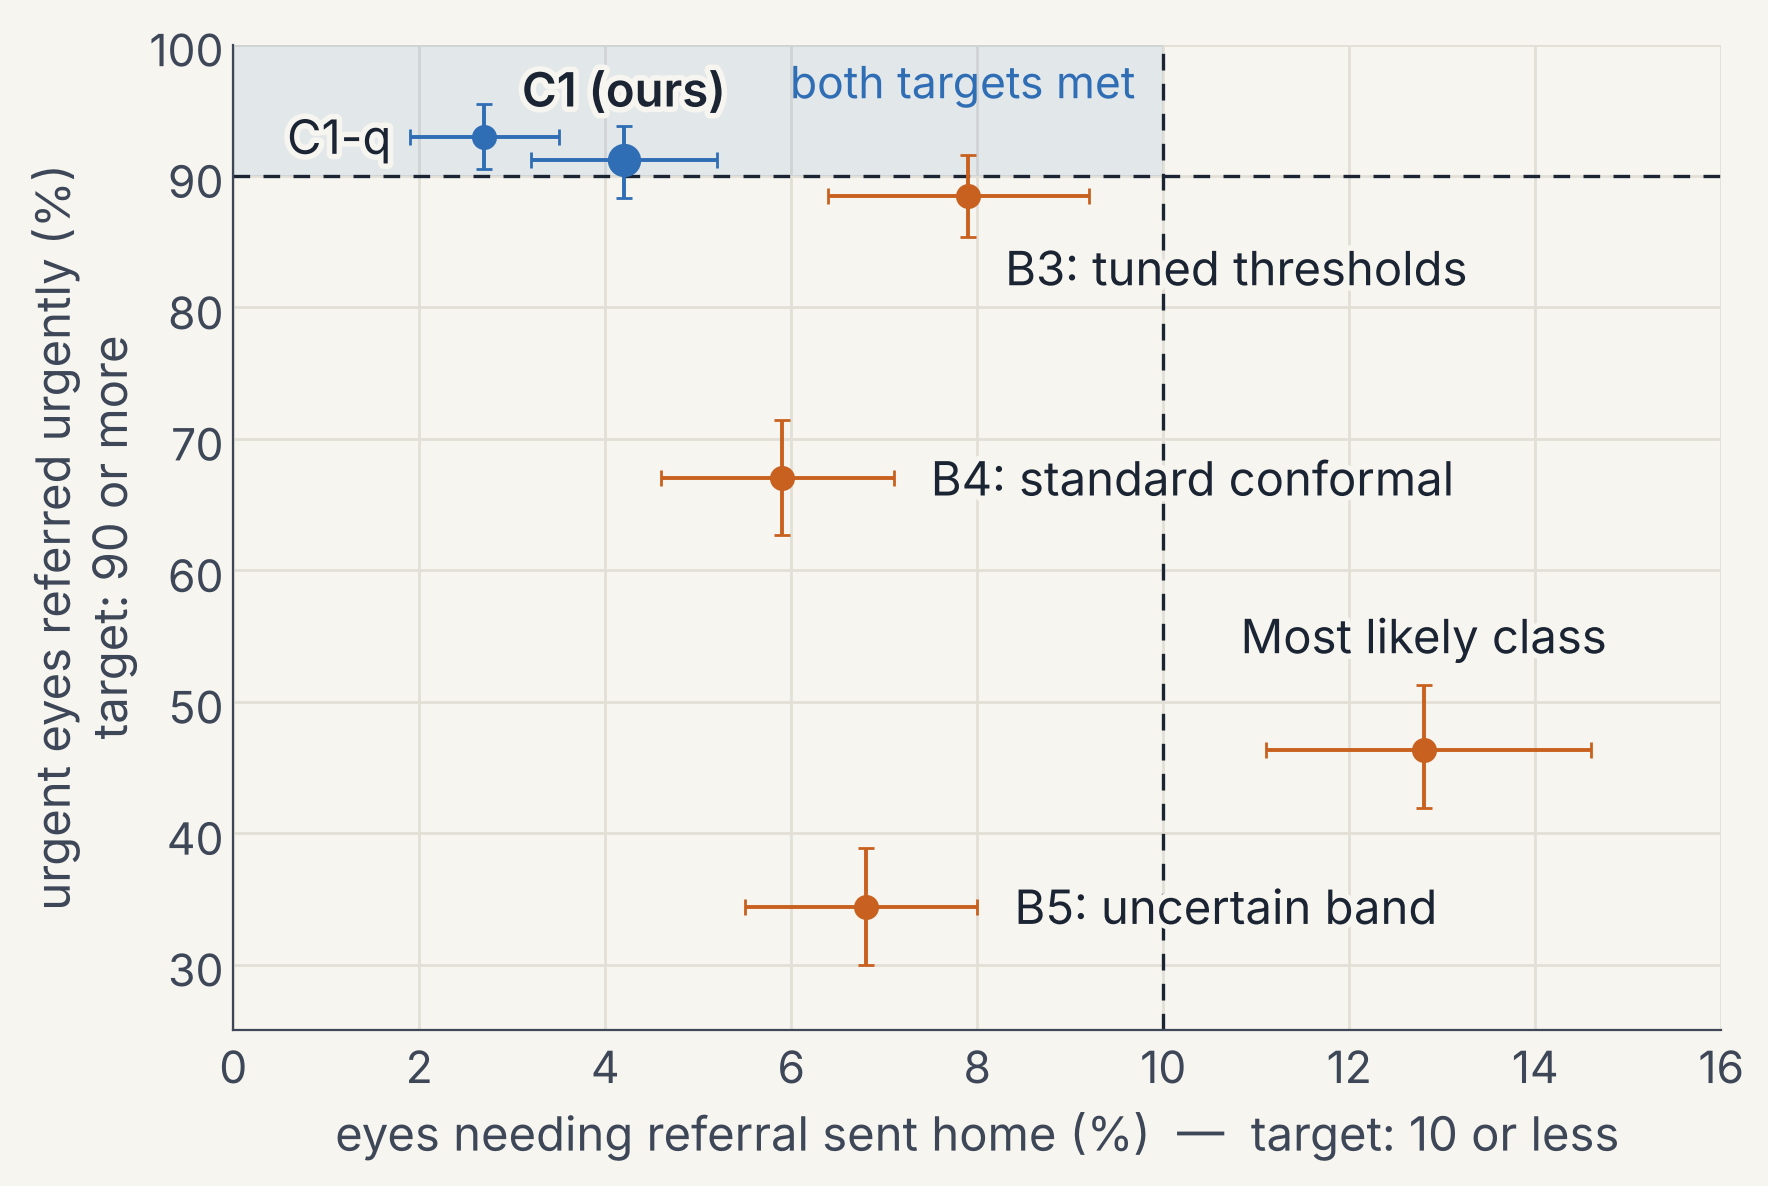
\includegraphics[width=0.9\linewidth]{fig/ch_c1_targets.png}
\caption{The two targets on APTOS for each rule (95\pct{} CIs; dashed: targets). Only C1 and C1-q meet both.}\label{fig:c1}
\end{figure}
The price is the urgent load (Tab.~\ref{tab:grade}): 336 urgent referrals per 1,000 eyes, only 36\pct{} truly urgent, because 64\pct{} of grade-2 eyes are flagged urgent (grade 0: 97.8\pct{} sent home; grades 3, 4: 91.7, 90.8\pct{} urgent). At $\alpha=0.05$, C1 sends home 2.4\pct{} and refers 96.5\pct{} urgently. Every course model meets both targets under C1; a better model sends more healthy eyes home (logistic regression 87.8\pct, naive Bayes 71.5\pct).

\subsection{C2 and E2: a new clinic needs labelled photos}
\begin{table}[t]\centering\small
\begin{tabular}{@{}llrcccc@{}}\toprule
Clinic & Rule & $k$ & Ref. & Urg. & Healthy & Unc.\\\midrule
IDRiD & B6 & -- & 10.6 & 87.2 & 75.5 & 2.3\\
 & C2 & 50 & 2.1 & 93.6 & 36.8 & 14.4\\
 & C2 & 300 & 4.8 & 90.7 & 51.0 & 15.5\\
 & B3-$k$ & 50 & 8.9 & 87.0 & 68.9 & 0.0\\
 & B4-$k$ & 50 & 6.6 & 82.1 & 57.8 & 27.3\\\midrule
Messidor-2 & B6 & -- & 79.8 & 32.8 & 97.9 & 1.2\\
 & C2 & 100 & 1.3 & 97.6 & 5.3 & 10.6\\
 & C2 & 300 & 6.2 & 92.5 & 25.5 & 43.5\\
 & B3-$k$ & 300 & 10.2 & 87.2 & 36.0 & 0.0\\
 & B4-$k$ & 300 & 29.4 & 57.0 & 65.9 & 36.8\\\bottomrule
\end{tabular}
\caption{New clinics (\%, mean over 200 draws of $k$ local photos; tested on the clinic's other photos). Columns as in Tab.~\ref{tab:c1}.}\label{tab:c2}
\end{table}
\begin{figure}[t]\centering
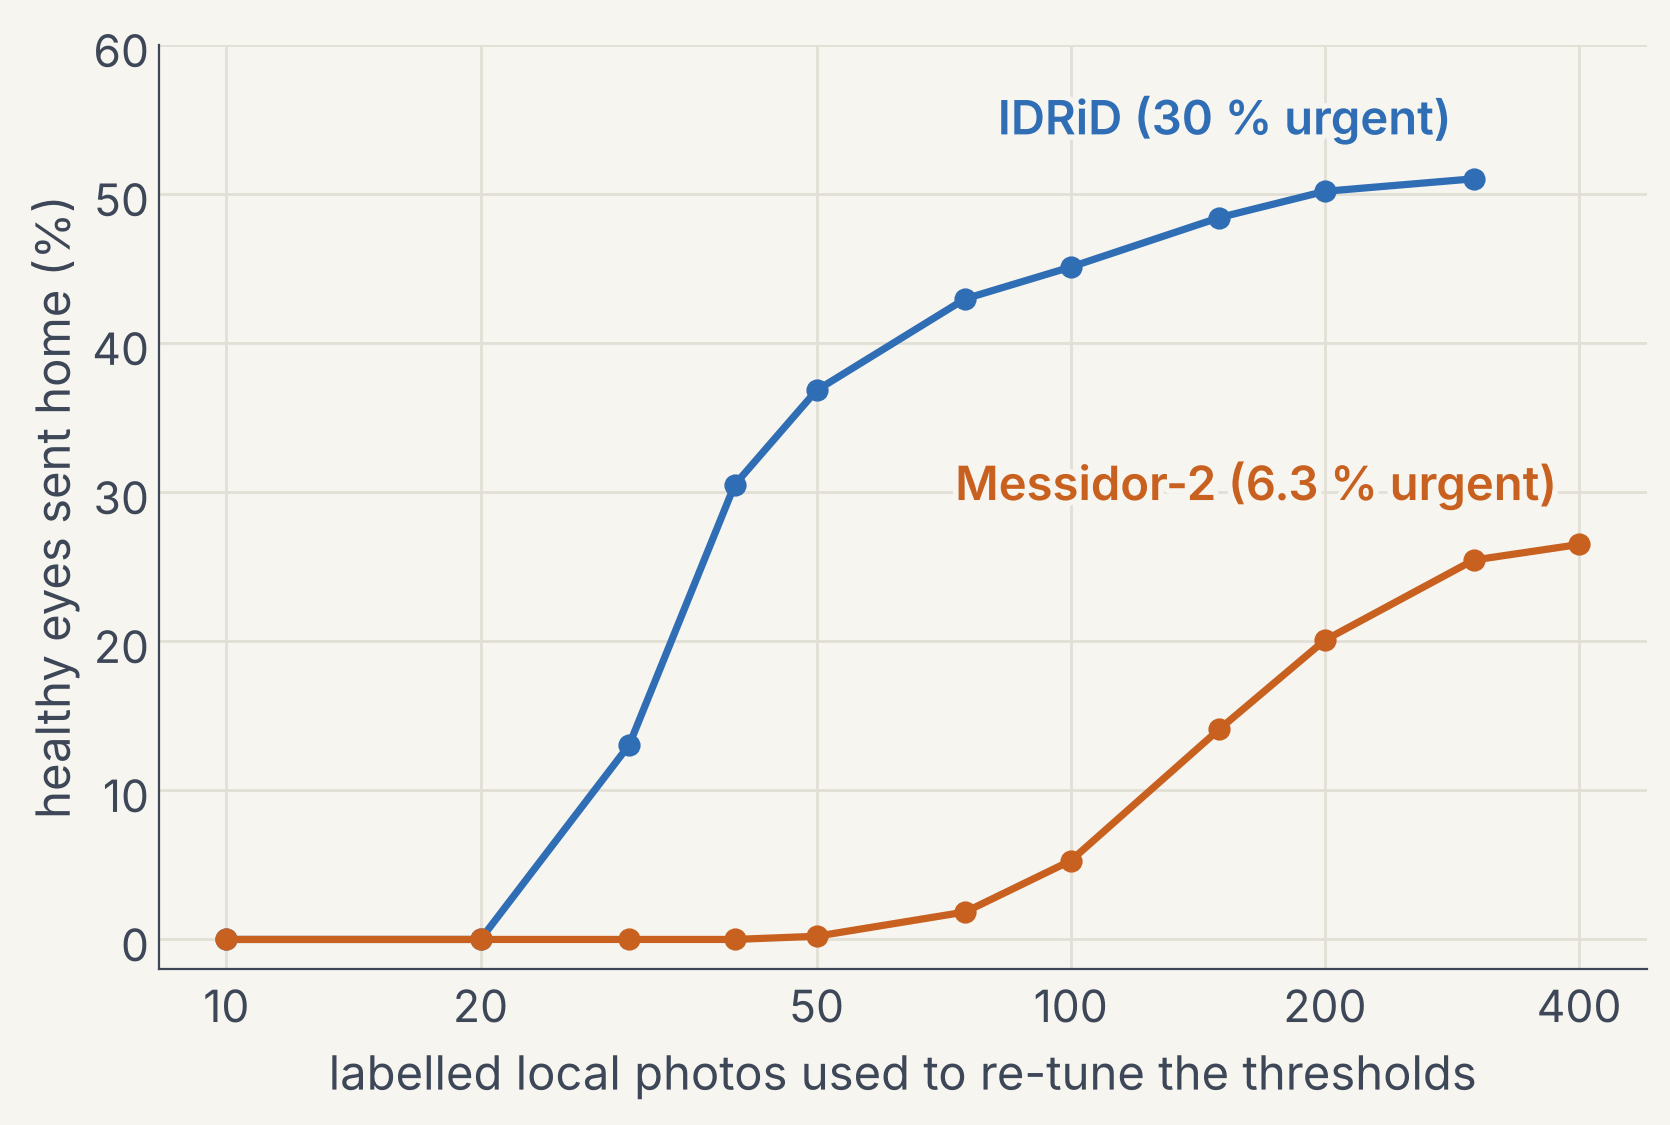
\includegraphics[width=0.92\linewidth]{fig/ch_c2_curves.png}
\caption{C2: healthy eyes sent home as the number of labelled local photos grows (mean over 200 draws); both targets hold at every $k$. The rarest class (urgent) decides when the curve leaves zero.}\label{fig:c2}
\end{figure}
With APTOS thresholds unchanged (B6), Messidor-2 sends home 80\pct{} of its referable eyes. Refitting the three thresholds restores both targets (Tab.~\ref{tab:c2}, Fig.~\ref{fig:c2}): every class's coverage averaged over draws is $\ge 89.9$\pct{} at every $k$. A class needs 9 local photos before its threshold is finite, so the urgent class decides: 30\pct{} of IDRiD eyes are urgent, only 6.3\pct{} of Messidor-2's. At Messidor-2 usefulness is capped by the APTOS model's ranking there (AUROC 0.764), not by the rule. Conformal beats tuning when photos are few (B3-$k$ refers 73\pct{} of urgent IDRiD eyes urgently at $k{=}10$, C2 100\pct). Retraining is no substitute: B7a refers 4--32\pct{} of Messidor-2's urgent eyes urgently and B7b still sends home 45--74\pct{} of its referable eyes.

On IDRiD's \emph{official} split C2 misses the urgent target (78--88\pct{} for $k\ge40$): its 32 urgent test eyes score lower than the training split's (median $P(\text{urgent})$ 0.28 vs 0.40, Mann--Whitney $p=0.15$). The guarantee needs calibration photos that resemble later ones.

\subsection{C3 and E3: prevalence and workload}
\begin{table}[t]\centering\small
\begin{tabular}{@{}lcccccc@{}}\toprule
Referable & Ref. & Urg. & /1000 & PPV & B4 all & B4 urg.\\\midrule
5\pct & 4.1 & 91.2 & 154 & 30.7 & 95.5 & 67.5\\
12.5\pct & 4.4 & 91.2 & 217 & 54.6 & 94.5 & 67.3\\
25\pct & 4.3 & 91.1 & 321 & 73.7 & 92.6 & 66.8\\
40.6\pct{} (APTOS) & 4.3 & 91.1 & 451 & 85.2 & 90.4 & 66.9\\\bottomrule
\end{tabular}
\caption{C1 under label shift (\%, 200 resamples of half of APTOS). B4's average coverage looks better as sick eyes get rarer while it still misses one urgent eye in three.}\label{tab:c3}
\end{table}
C1's targets hold at every prevalence, while referrals fall from 451 to 154 per 1,000 and the PPV of a referral from 85.2 to 30.7\pct{} (Tab.~\ref{tab:c3}). Without correction (B8) the forecast at 5\pct{} is 297 referrals per 1,000 too many; with EM shares the error is 6--11 per 1,000, as small as with the true shares (B9, 10--12). EM estimates 5.4\pct{} referable when the truth is 5\pct, and the Bayes adjustment cuts the ECE of $P(\text{referable})$ from 0.092 to 0.012. At real clinics EM fails because more than the shares changes (Messidor-2: 99.5\pct{} no-referral estimated vs 73.8\pct); the $k$ labelled photos C2 needs anyway forecast C2's workload to $+7$ per 1,000.

\subsection{Errors, ablations, robustness}
\begin{table*}[t]\centering\small
\begin{tabular}{@{}lcc@{}}\toprule
Subgroup & Referable sent home & Urgent not urgent\\\midrule
All APTOS eyes & 4.2 (63/1,487) & 8.8 (43/488)\\
Camera group H (55 ref., 15 urg.) & 47.3 (34.7--60.2) & 6.7 (1.2--29.8)\\
Camera group M & 3.8 (2.6--5.4) & 8.9 (6.1--12.8)\\
Camera group S & 1.4 (0.8--2.6) & 8.8 (5.6--13.7)\\
Sharpest third & 9.4 (6.4--13.5) & 5.3 (2.3--11.9)\\
Least sharp third & 3.3 (2.2--4.9) & 10.5 (7.1--15.2)\\
Quality warning & 4.0 (1.6--9.8) & 5.1 (1.4--16.9)\\
Copies with another class & 6.7 (2.3--17.9) & 9.5 (2.7--28.9)\\\bottomrule
\end{tabular}
\caption{C1's errors by subgroup (\%, 95\pct{} Wilson intervals).}\label{tab:err}
\end{table*}
\begin{table*}[t]\centering\small
\begin{tabular}{@{}llccccc@{}}\toprule
Test photos & Thresh. & AUROC & Ref. & Urg. & Healthy & Unc.\\\midrule
original & orig. & 0.973 & 4.2 & 91.2 & 87.8 & 1.0\\
blur 3\,px & orig. & 0.918 & 8.2 & 96.5 & 73.5 & 0.5\\
blur 3\,px & blurred & 0.918 & 3.6 & 91.4 & 49.1 & 23.0\\
half bright. & orig. & 0.969 & 6.7 & 87.1 & 88.6 & 2.0\\
half bright. & dark & 0.969 & 5.0 & 91.8 & 86.4 & 2.3\\
JPEG q20 & orig. & 0.945 & 2.9 & 93.0 & 69.7 & 1.1\\
JPEG q20 & JPEG & 0.945 & 1.7 & 89.1 & 65.0 & 10.6\\\midrule
\multicolumn{2}{@{}l}{512\,px features} & 0.975 & 4.4 & 91.0 & \multicolumn{2}{l}{Mess.\ AUROC 0.782}\\
\multicolumn{2}{@{}l}{Graham filter} & 0.970 & 4.0 & 93.2 & \multicolumn{2}{l}{Mess.\ AUROC 0.747}\\\bottomrule
\end{tabular}
\caption{Robustness (C1 thresholds from original or equally degraded calibration photos) and image ablations (\%). JPEG's 89.1\pct{} is within the noise of 488 urgent eyes ($\pm2.8$).}\label{tab:abl}
\end{table*}
C1's errors concentrate in one subgroup (Tab.~\ref{tab:err}): on APTOS's mostly-healthy (H) cameras it sends home 26 of 55 referable eyes (47.3\pct, CI 34.7--60.2), against 3.8\pct{} and 1.4\pct{} on mixed (M) and mostly-sick (S) cameras. The 43 missed urgent eyes are confident misses (median $P(\text{urgent})$ 0.058 vs 0.424). Of the 63 referable eyes sent home, 52 are grade 2, closest to the boundary. Sharpness is tangled with the camera: 21 of the sharpest third's 25 errors come from H cameras. One threshold per camera group cannot be fitted from a fold's calibration photos (about 5 routine and 2 urgent H-camera photos per fold, below 9). In the ablations (Tab.~\ref{tab:abl}), 512\,px features help a little at Messidor-2 (AUROC 0.782 vs 0.760); Ben Graham's filter and PCA size do not matter. Blur doubles referable eyes sent home (8.2\pct) and half brightness drops urgent referral to 87.1\pct{} with thresholds from good photos; recalibrating on equally poor photos restores both targets at a cost in usefulness (blur: 49.1\pct{} of healthy eyes sent home, 23\pct{} to a grader).

\section{Additional work: does the guarantee hold for every group?}\label{sec:extra}
C1 promises coverage per class, on average over the eyes it is calibrated on. We ask whether it holds for every camera, every new clinic and every orientation of the photo, and what restores it where it fails.

\textbf{The camera shortcut}~\cite{geirhos}. We group APTOS cameras (photo sizes) by their share of referable eyes: H ($\le$10\pct: 1,612 photos, 55 referable), M (1,298, 55\pct), S ($\ge$80\pct: 752). Probes trained on grade-0 eyes alone recognise the camera from the features with 91.1\pct{} balanced accuracy (5 cameras, chance 20\pct) and separate H cameras perfectly. Every Messidor-2 photo scores above 0.5 on a probe for H-camera style.

\textbf{Eleven methods compared.} Every method is logistic regression on the same features with $C{=}0.003$, retrained in E1's folds, with C1 on each fold's calibration photos. \emph{Ours} weights each training photo by $P(\text{class})/P(\text{class}\mid\text{camera group})$, so that in the weighted data the camera says nothing about the class. Baselines: group-balanced weights~\cite{sagawa,idrissi}, DFR~\cite{kirichenko}, Group DRO~\cite{sagawa}, JTT ($\times5$, $\times20$)~\cite{jtt}, per-group thresholds (fold calibration, or cross-fitted from the other folds), and LEACE erasure~\cite{leace} fitted on healthy eyes or within grade.

\begin{table}[t]\centering\small
\begin{tabular}{@{}lcccc@{}}\toprule
Method & Worst grp. & Urg. & Healthy & vs ours\\
 & ref.\ home & worst & home & saved/lost\\\midrule
Plain training & 43.6 (31--57) & 91.8 & 87.6 & 0/19\\
\textbf{Decorrelated (ours)} & \textbf{9.1} (4--20) & 91.1 & \textbf{84.3} & --\\
Group-balanced & 5.5 (2--15) & 91.8 & 76.7 & 2/0\\
Group DRO & 3.6 (1--12) & 91.4 & 70.7 & 3/0\\
DFR & 3.9 (3--6) & 91.2 & 26.4 & 5/0\\
JTT $\times5$ & 21.8 (13--34) & 86.7 & 81.4 & 0/7\\
JTT $\times20$ & 7.3 (3--17) & 86.7 & 63.5 & 2/1\\
Per-group thr., fold & 2.2 (1--4) & 93.6 & 15.8 & 5/0\\
Per-group thr., cross-fit & 7.3 (3--17) & 90.2 & 75.8 & 1/0\\
LEACE, healthy & 52.7 (40--65) & 90.7 & 88.1 & 0/24\\
LEACE, within grade & 36.4 (25--50) & 91.8 & 85.9 & 1/16\\\bottomrule
\end{tabular}
\caption{The camera subgroup (\%, APTOS out of fold). Worst group is H unless DFR (S) or fold thresholds (M). Last column: H-camera referable eyes the method refers and ours sends home, and the reverse (exact McNemar).}\label{tab:fair}
\end{table}
\begin{figure}[t]\centering
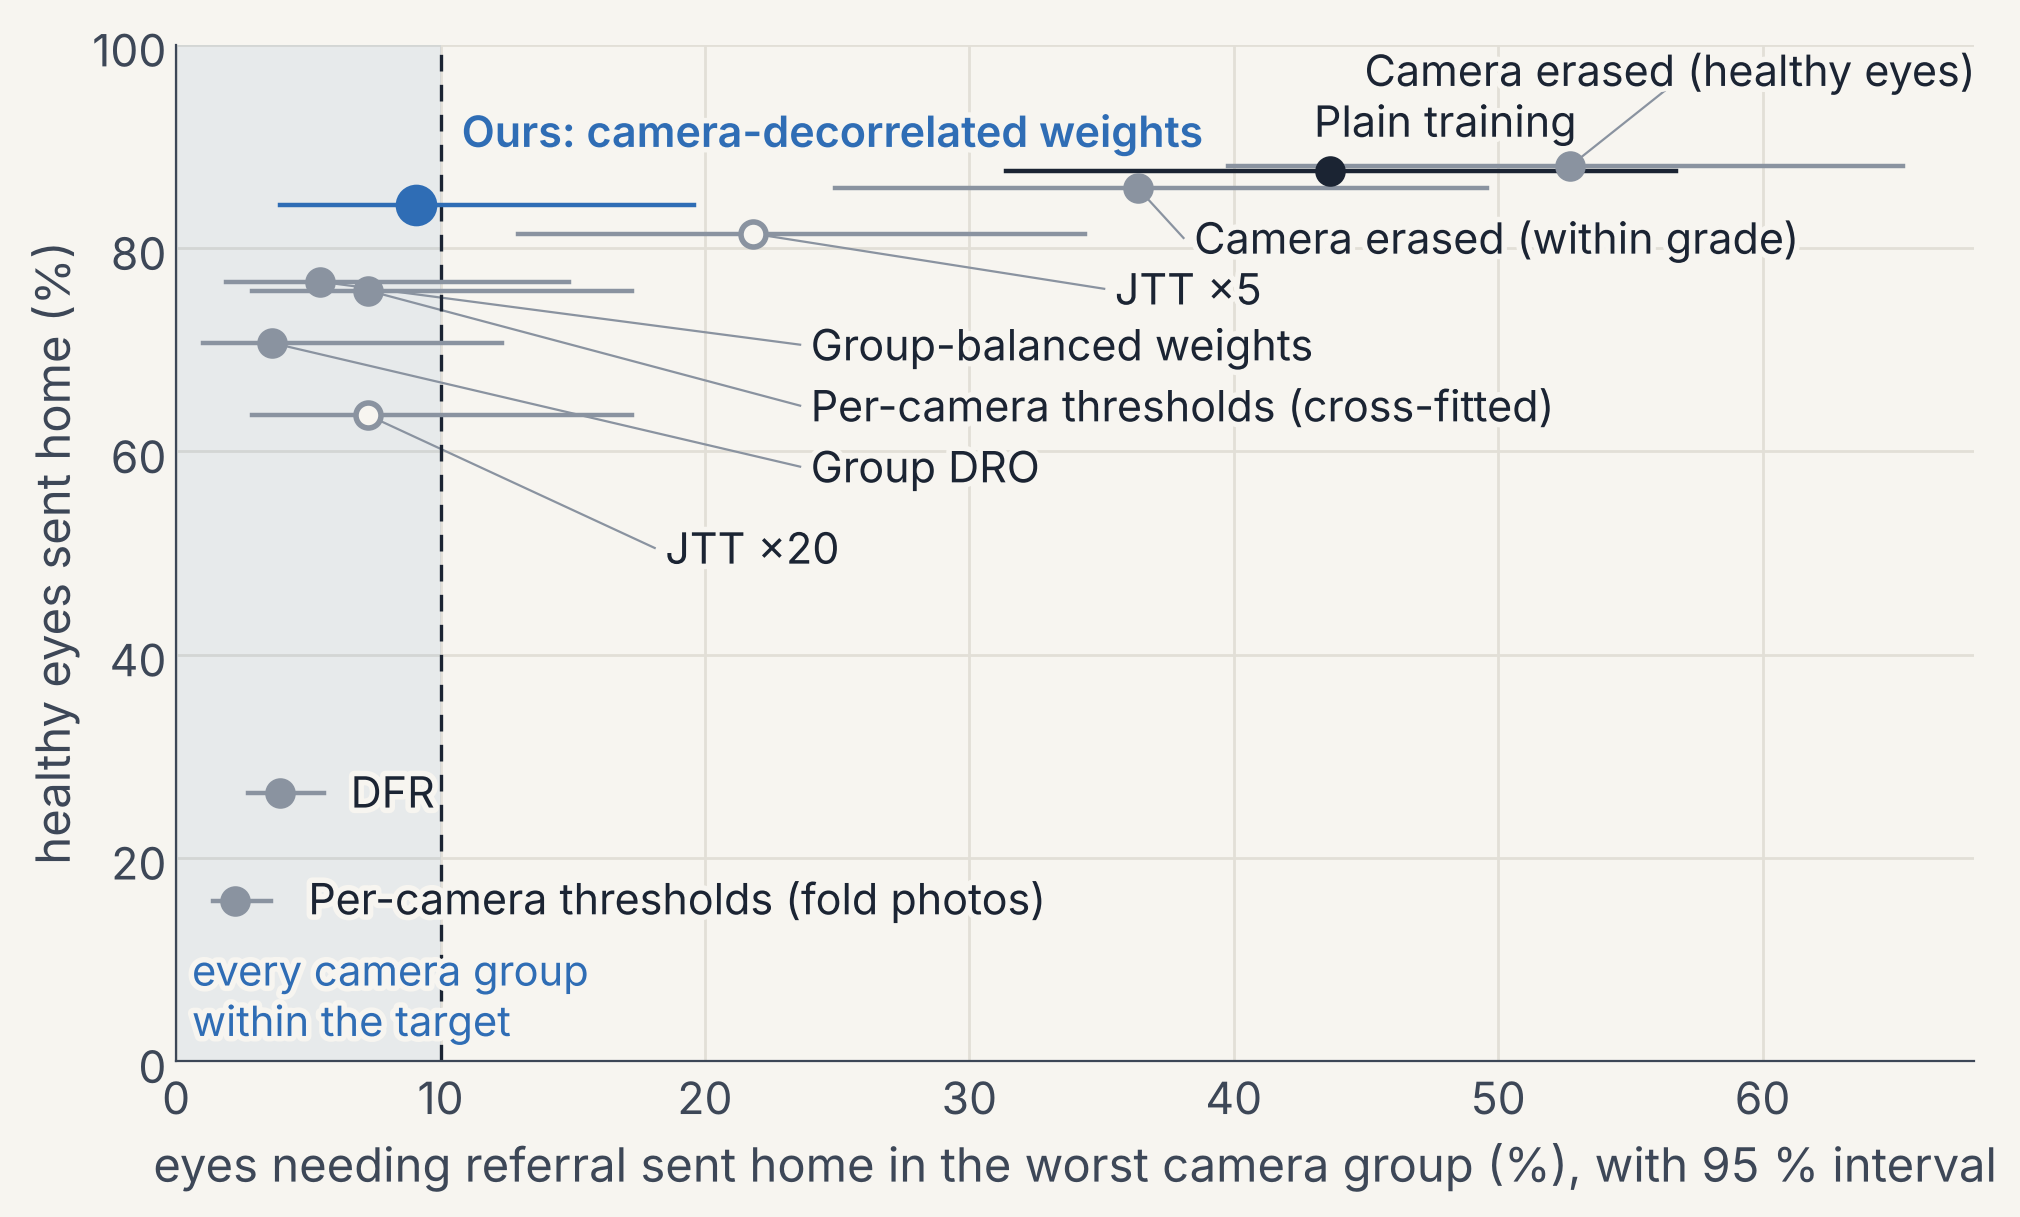
\includegraphics[width=\linewidth]{fig/ch_camera_tradeoff.png}
\caption{Fairness against usefulness: worst camera group's referable eyes sent home (95\pct{} Wilson interval) against all healthy eyes sent home. Shaded: every group meets the 10\pct{} target. Hollow: urgent target missed in the worst group.}\label{fig:fair}
\end{figure}
Six methods meet both targets in every camera group (Tab.~\ref{tab:fair}, Fig.~\ref{fig:fair}); each saves significantly more H-camera referable eyes than plain training (exact McNemar, $p\le4\times10^{-6}$), and with 55 such eyes none is significantly better than ours ($p\ge0.06$). Ours costs the fewest healthy eyes (84.3\pct; each other passing method sends home significantly fewer, $p\le3\times10^{-45}$). Even with each baseline's own knob swept and the best setting chosen with hindsight, ours leads (group-balanced at strength 0.75: 80.5\pct; Group DRO 76.0\pct; no JTT setting meets both targets). The weights make the 55 sick H-camera eyes count 11--14 times the average photo, lifting the median $P(\text{referable})$ of H-camera grade-2 eyes from 0.15 to 0.64. Erasure makes the camera unreadable in healthy eyes (probe AUROC $1.000\to0.500$) but not in referable ones, so the misses stay: changing what the data teach works, hiding the camera does not. No method makes APTOS thresholds work at a new clinic (36--52\pct{} of Messidor-2's urgent eyes referred urgently).

\textbf{Exact evidence maps.} Because logistic regression is linear in average-pooled features, each log-odds splits exactly into a $7{\times}7$ map~\cite{cam} (error $<4\times10^{-7}$). 71\pct{} of the H-vs-M camera gap in routine log-odds of grade-2 eyes ($-1.36$ vs $+1.60$) lies inside the retina (Fig.~\ref{fig:maps}); the reweighted model shrinks it to 0.60 by finding evidence inside H-camera retinas. A deletion test~\cite{rise} confirms the maps: blurring the 4 most urgent cells lowers the urgent log-odds by 1.51, against 0.56 for random retina cells. A fixed top-left hotspot of the network, stable under mirroring, is plausibly due to asymmetric zero padding~\cite{pad}.

\begin{figure}[t]\centering
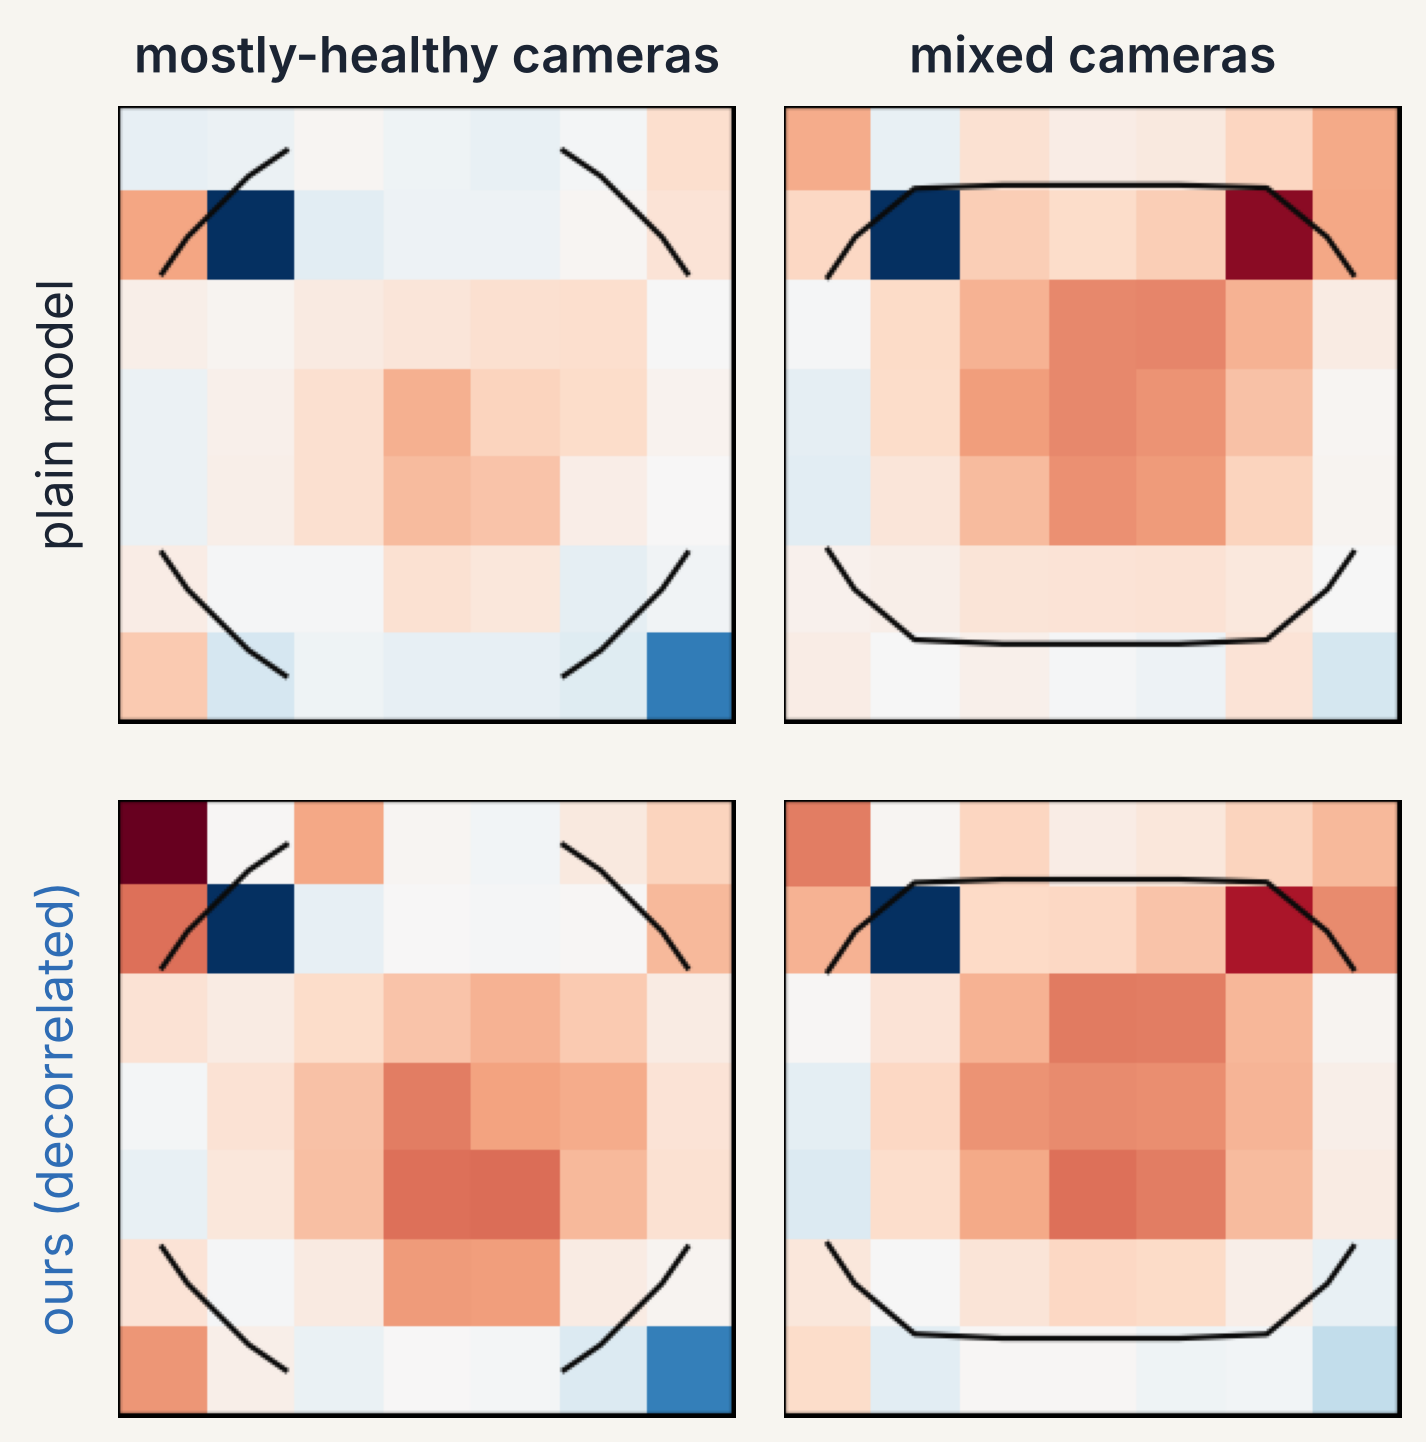
\includegraphics[width=0.72\linewidth]{fig/ch_evidence_maps.png}
\caption{Mean exact evidence of APTOS grade-2 eyes for routine against no referral per $7{\times}7$ cell (red: towards referral; line: retina edge). On H cameras the plain model finds little evidence in the retina; the decorrelated model finds it there, as on mixed cameras. Averages only; no individual photo is shown.}\label{fig:maps}
\end{figure}
\textbf{Mirror-averaged features.} Mirroring a photo changes C1's decision for 11.0\pct{} of APTOS eyes. Averaging the features of a photo and its mirror image makes every decision orientation-independent, at equal or better AUROC (0.974/0.924) with both targets still met.

\textbf{C2-IW: label-efficient recalibration (new method).} C2 needs 9 labelled photos of the rarest class before any healthy eye is sent home. C2-IW labels the photos most likely to be rare and undoes the bias with weights. Rarity $r(x)=\sum_c p(c\mid x)/m_c$, with $m_c$ the clinic mean of $p(c\mid x)$, is mixed with uniform sampling, $r'=(1-\lambda)+\lambda r/3$ (a defensive mixture~\cite{hesterberg}). Each exam is labelled independently with probability $\pi\propto r'$ ($k$ labels on average), labelled photos get weights $w=1/\pi$, and each class threshold is the weighted $(1-\alpha)(1+1/n_{\text{eff}})$ quantile with Kish's effective size $n_{\text{eff}}=(\sum w)^2/\sum w^2$~\cite{kish}. With equal weights this is exactly C2; in general it is the weighted conformal threshold~\cite{tibshirani} with the test weight replaced by its expectation $\sum w^2/\sum w$, so coverage is approximate. The idea follows active inference~\cite{zrnic}. We use $\lambda=0.25$, the largest value on the grid within noise of 90\pct{} everywhere (every $\lambda$ is shown).

\begin{figure*}[t]\centering
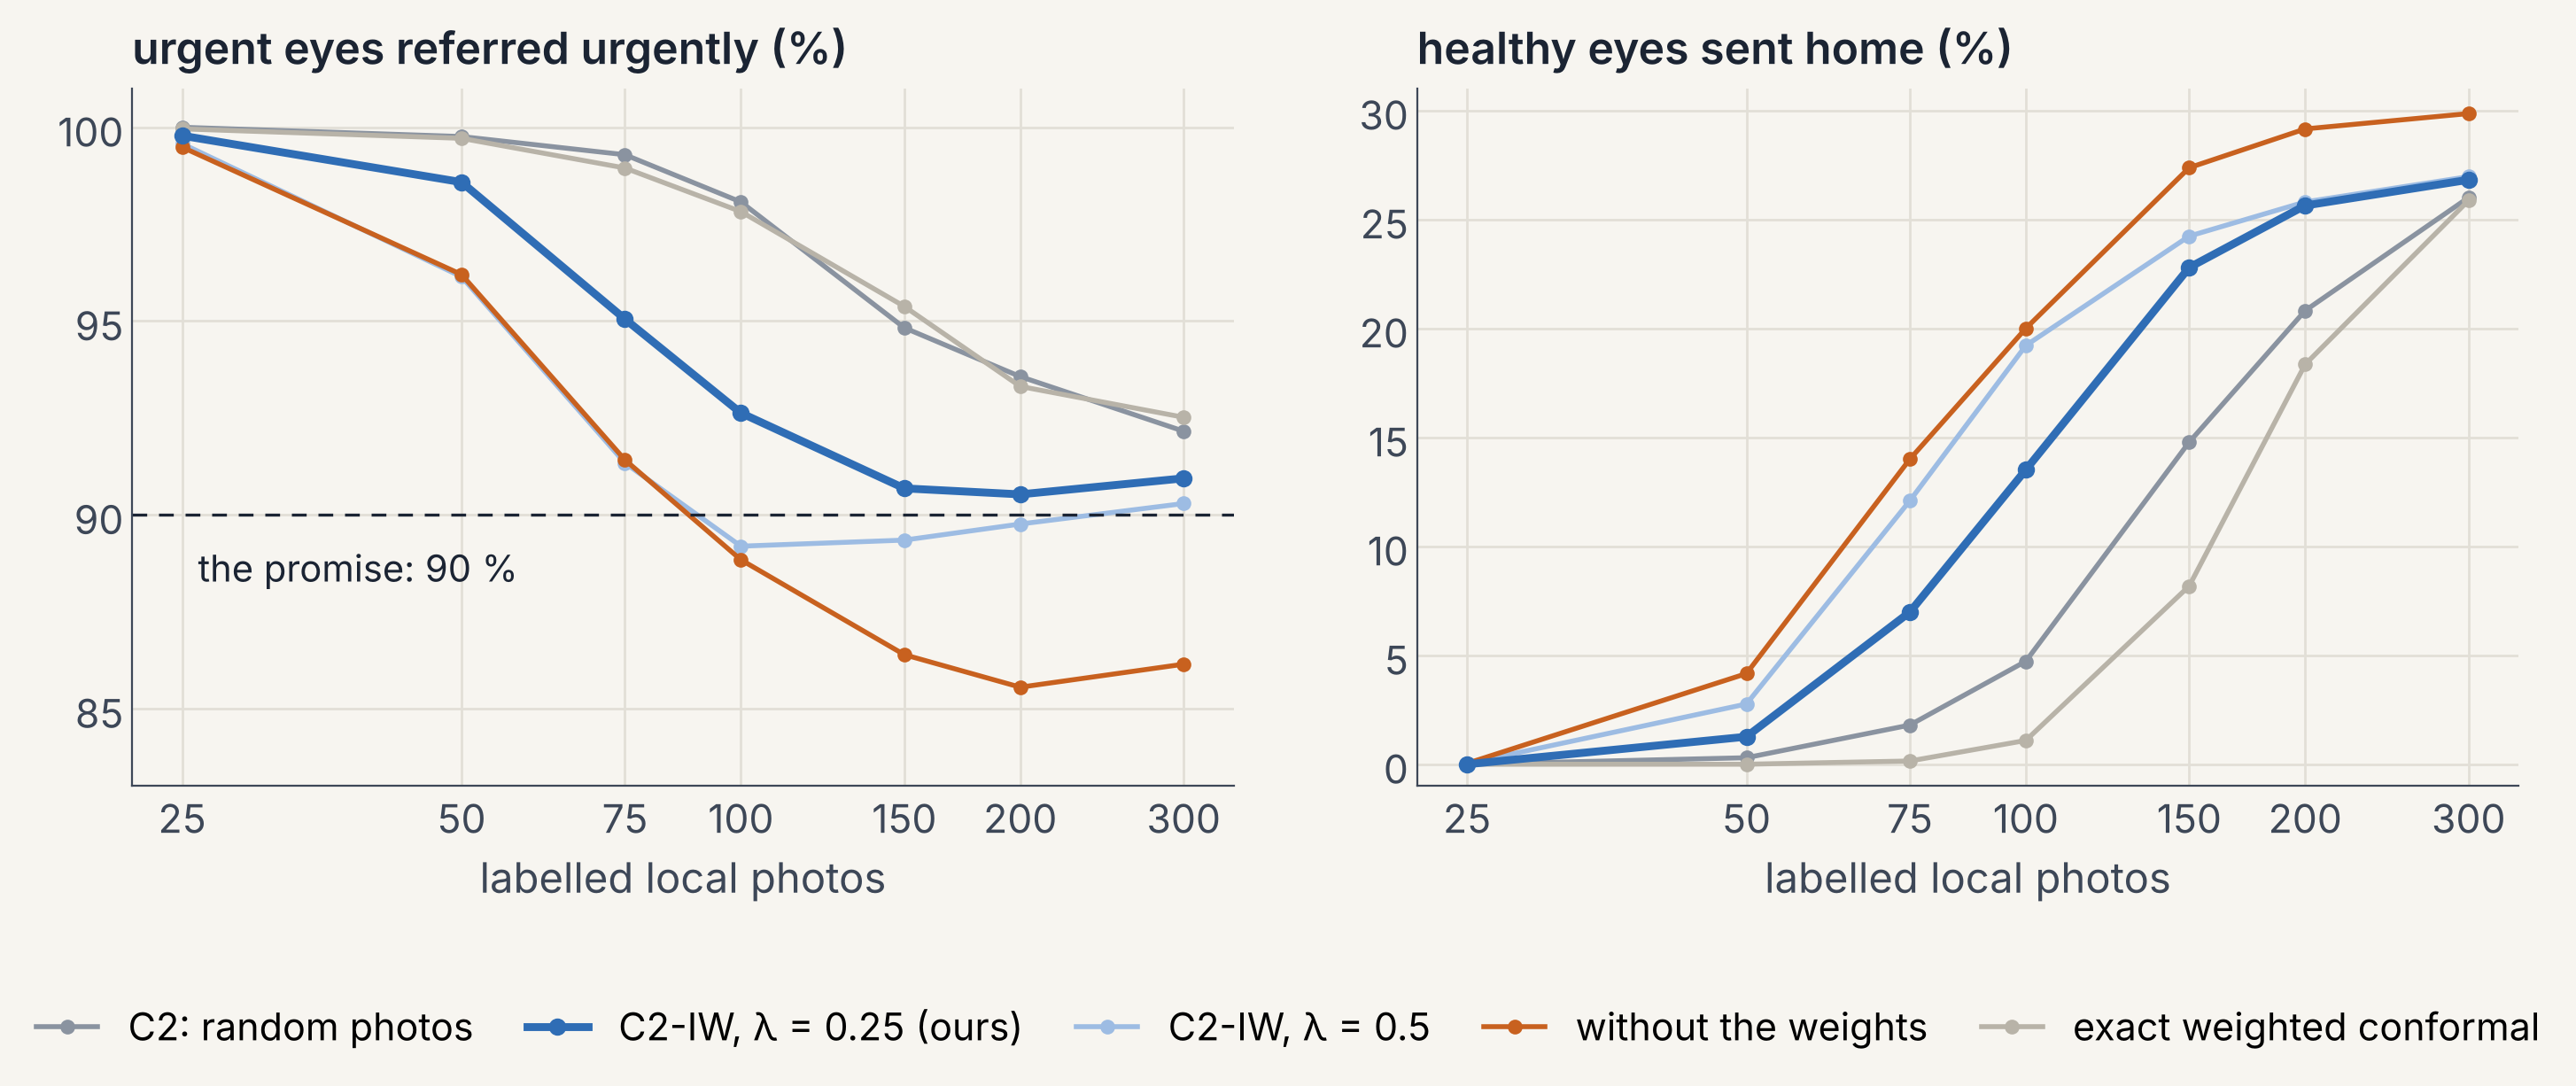
\includegraphics[width=0.82\linewidth]{fig/ch_c2iw.png}
\caption{C2-IW at Messidor-2 (1,000 draws, tested on a held-out half of the clinic): urgent eyes referred urgently (left) and healthy eyes sent home (right) as the label budget grows. Without the weights, coverage falls to 85.6--88.8\pct.}\label{fig:c2iw}
\end{figure*}
\begin{table}[t]\centering\small
\resizebox{\linewidth}{!}{\begin{tabular}{@{}lcccccc@{}}\toprule
 & \multicolumn{2}{c}{Mess., 100} & \multicolumn{2}{c}{Mess., 150} & \multicolumn{2}{c}{APTOS 5\pct, 300}\\
Method & Urg. & Healthy & Urg. & Healthy & Urg. & Healthy\\\midrule
C2, random & 98.1 & 4.7 & 94.8 & 14.8 & 99.4 & 3.4\\
\textbf{C2-IW, $\lambda{=}0.25$} & 92.6 & \textbf{13.5} & 90.7 & \textbf{22.8} & 91.6 & \textbf{62.8}\\
C2-IW, $\lambda{=}0.5$ & 89.2 & 19.2 & 89.3 & 24.2 & 91.0 & 82.4\\
No weights & 88.8 & 20.0 & 86.4 & 27.4 & 89.8 & 73.9\\
Exact weighted~\cite{tibshirani} & 97.8 & 1.1 & 95.4 & 8.2 & 97.9 & 0.0\\\bottomrule
\end{tabular}}
\caption{C2-IW (\%, 1,000 draws; Monte Carlo SE of the urgent columns $\le0.4$). C2-IW sends home at most 6.8\pct{} of referable eyes.}\label{tab:c2iw}
\end{table}
At $\lambda=0.25$ mean urgent coverage is $\ge90.5$\pct{} at every budget in every setting (Tab.~\ref{tab:c2iw}, Fig.~\ref{fig:c2iw}). At Messidor-2, C2-IW sends home 13.5\pct{} of healthy eyes with 100 labels, which C2 needs about 150 for, and 25.6\pct{} with 200, which C2 needs 300 for. At 5\pct{} prevalence, with 300 labels it sends home 62.8\pct{} against 3.4\pct{} for C2. At IDRiD (30\pct{} urgent) there is nothing to gain. The weights are essential: the urgent threshold is set by the 10\pct{} of urgent eyes that look healthy, which rarity sampling under-samples.

\textbf{Smaller extensions.} C1-g sends sets holding urgent and another class to a grader: urgent referrals fall from 336 to 58 per 1,000 (68\pct{} truly urgent) with 28.8\pct{} of eyes to a grader. C2-PAC uses the training-conditional bound~\cite{vovk} so that a single clinic's coverage falls below 90\pct{} in at most 10\pct{} of draws (observed $\le6$\pct, C2 up to 36\pct). BBSE~\cite{bbse} estimates shares as EM does, with a wider spread.

\section{Discussion and limitations}
Class-wise thresholds are necessary: one threshold (B4) refers only 67\pct{} of urgent eyes urgently. Every clinic needs its own labelled photos, 50 at IDRiD and 200--300 at Messidor-2, about a third fewer with C2-IW. Exchangeability is the assumption to watch (IDRiD's official split). Safety costs workload, which C3 forecasts. A guarantee per class is not a guarantee per subgroup. \begin{table*}[t]\centering\small
\begin{tabular}{@{}p{0.25\linewidth}p{0.38\linewidth}p{0.33\linewidth}@{}}\toprule
Limitation & Effect & What we did\\\midrule
Frozen ImageNet features, 224\,px & poor ranking at Messidor-2 (0.764) caps usefulness & 512\,px ablation; fine-tuning left open\\
No patient IDs in APTOS & two eyes may straddle folds & copies and look-alikes grouped\\
Guarantee is an average over draws & single IDRiD draws meet both targets 60--77\pct{} of the time & C2-PAC per-clinic promise\\
Exchangeability assumed & IDRiD official split misses urgent target & flagged and examined\\
Camera known only via photo size & a proxy & treated as a proxy\\
55 referable H-camera eyes & wide CIs (ours 4--20\pct) & Wilson CIs, exact McNemar\\
C2-IW coverage approximate & $\lambda\ge0.5$ up to 3 points short & 1,000 draws, all $\lambda$ shown\\\bottomrule
\end{tabular}
\caption{Limitations.}\label{tab:lim}
\end{table*}
\emph{Limitations} (Tab.~\ref{tab:lim}): frozen 224\,px ImageNet features limit ranking at new clinics (Messidor-2 AUROC 0.764); APTOS has no patient IDs, so two eyes of a patient may fall in different folds; 51 APTOS copies carry conflicting grades; guarantees are averages over calibration draws (C2-PAC addresses this); the camera is known only through photo size; the H-camera interval for ours (4--20\pct) does not show it below 10\pct; C2-IW's coverage is shown by simulation, not proven, and $\lambda$ was chosen on the grid it is judged on; each experiment is one run with fixed seeds. Fine-tuning on fundus photos is the main future step.

\section{Reproducibility}
\textbf{Declaration.} Every number, table and figure in this report was produced by the code at \url{https://github.com/Nova1369/dr-referral-triage}, at the commits in Tab.~\ref{tab:commits}, from the public datasets listed in \texttt{data/README.md}, without manual editing. \texttt{bash run\_all.sh} regenerates them (about 3 hours on a laptop CPU, no GPU). Seeds are fixed (42); model settings are chosen in inner folds, thresholds on calibration photos only, and new clinics are used only for calibration draws and testing.

\textbf{Artifacts.} \texttt{requirements.txt} pins the exact versions (Python 3.13.16, numpy 2.5.3, pandas 3.0.5, scikit-learn 1.9.1, scipy 1.18.1; torch 2.7.1 for features), with \texttt{environment.yml} for conda. Checkpoints: the final logistic regression and its standardiser (\texttt{checkpoints/lr\_aptos\_ref3.npz}, 55\,kB; \texttt{export\_checkpoint.py check} reproduces it to $6\times10^{-7}$); the 102\,MB ResNet-50 backbone is linked (timm release \texttt{resnet50\_ram-a26f946b.pth}, SHA-256 \texttt{a26f946b\dots a3e7}) and checked by \texttt{scripts/download\_weights.sh}. Datasets are not included (Messidor-2 licence); aggregate reference outputs are in \texttt{results/}, and \texttt{scripts/compare\_results.py} diffs a re-run. A second machine (Linux ARM, Python 3.10, scikit-learn 1.7) reproduced C1, C3, the error analysis and C2-IW identically, E2 within 0.1 points and the camera benchmark within about 1 point.

\begin{table*}[t]\centering
\begin{minipage}[t]{0.495\textwidth}\centering\scriptsize
\begin{tabular}{@{}r@{\hspace{4pt}}l@{\hspace{4pt}}l@{\hspace{4pt}}p{0.5\linewidth}@{}}\toprule
\# & Commit & Date (IST) & Message\\\midrule
1 & \texttt{eb7ccc49ce} & 2026-10-25 00:39 & Preprocessing: retina crop, quality checks, duplicate groups, folds\\
2 & \texttt{9ed58ff619} & 2026-10-25 02:29 & Frozen ResNet-50 feature extraction\\
3 & \texttt{e3a47c07ab} & 2026-10-25 09:49 & Add requirements.txt\\
4 & \texttt{85607c91ba} & 2026-10-25 10:25 & E1: nested CV for the course models and baselines\\
5 & \texttt{5b03e5c542} & 2026-10-25 10:28 & E0: standard conformal prediction at IDRiD and Messidor-2\\
6 & \texttt{51e23b0020} & 2026-10-25 11:29 & E1 summary tables; E0 results\\
7 & \texttt{e711fbd545} & 2026-10-25 11:30 & E1 results\\
8 & \texttt{7b233b7f2d} & 2026-10-25 11:32 & k-means check\\
9 & \texttt{30ae183824} & 2026-10-25 11:58 & Camera shortcut study\\
10 & \texttt{57e9d73397} & 2026-10-25 12:14 & run\_all.sh: every step in order\\
11 & \texttt{5a2082b6dd} & 2026-10-25 12:16 & Pipeline notes\\
12 & \texttt{328064940c} & 2026-11-03 21:31 & C1 class-wise referral rule; error analysis\\
13 & \texttt{91a9b7c2cd} & 2026-11-04 01:27 & Ablations and robustness checks\\
14 & \texttt{597b1fffd1} & 2026-11-04 01:30 & C1 results\\
15 & \texttt{b60cfed70b} & 2026-11-04 01:36 & C3: prevalence shift and workload forecast\\
16 & \texttt{9821a6f003} & 2026-11-04 02:04 & Ablation and robustness results\\
17 & \texttt{437ef23817} & 2026-11-04 02:18 & C2/E2: recalibration at new clinics, C2-PAC\\
18 & \texttt{98eb9b7b44} & 2026-11-04 02:19 & Update requirements\\
19 & \texttt{e8abf8148e} & 2026-11-04 10:26 & Camera fixes tuned under the E1 protocol\\
\bottomrule
\end{tabular}
\end{minipage}\hfill
\begin{minipage}[t]{0.495\textwidth}\centering\scriptsize
\begin{tabular}{@{}r@{\hspace{4pt}}l@{\hspace{4pt}}l@{\hspace{4pt}}p{0.5\linewidth}@{}}\toprule
\# & Commit & Date (IST) & Message\\\midrule
20 & \texttt{bd70ea68dd} & 2026-11-04 10:29 & E2 results\\
21 & \texttt{9f82faac80} & 2026-11-04 16:43 & Exact evidence maps, deletion and mirror tests\\
22 & \texttt{6ea7da0aa9} & 2026-11-04 18:35 & Feature variants, including mirrored photos\\
23 & \texttt{fb76710b1f} & 2026-11-04 20:33 & Mirror-averaged features\\
24 & \texttt{92ed8b00ef} & 2026-11-05 01:24 & Camera-group benchmark against strong baselines\\
25 & \texttt{e5f8ea8728} & 2026-11-05 01:33 & Camera-group benchmark results\\
26 & \texttt{200fe582cb} & 2026-11-05 01:34 & C2-IW: label-efficient recalibration\\
27 & \texttt{f951cadde0} & 2026-11-05 01:56 & Baseline sweeps at matched fairness\\
28 & \texttt{4d1a577322} & 2026-11-05 02:01 & C2-IW results\\
29 & \texttt{08984095a7} & 2026-11-05 02:01 & Update run\_all.sh and notes for the new studies\\
30 & \texttt{c4f93ae586} & 2026-11-08 17:09 & Restructure as a repository: src/, docs/, results/\\
31 & \texttt{45ff75397b} & 2026-11-08 17:10 & Export the final model as a small checkpoint\\
32 & \texttt{3b44f9fb50} & 2026-11-08 17:10 & run\_all.sh for the repository layout\\
33 & \texttt{520c2bd6bd} & 2026-11-08 17:10 & Pin the environment; weight download and result comparison scripts\\
34 & \texttt{8ee80c8ef1} & 2026-11-08 17:11 & Notes for data, checkpoints and results; MIT licence\\
35 & \texttt{01d5099164} & 2026-11-08 17:11 & README: setup, reproduction, layout\\
36 & \texttt{9abb423e78} & 2026-11-08 17:12 & Reproducibility statement\\
37 & \texttt{034205e71c} & 2026-11-08 17:12 & Leakage check for the E1 splits\\
\bottomrule
\end{tabular}
\end{minipage}
\caption{Commit history of the repository up to the code freeze (branch \texttt{main}; short hashes, dates in IST). The commit that adds this report comes next and is listed, with full hashes, in the README.}\label{tab:commits}
\end{table*}

\textbf{Acknowledgement.} Messidor-2 images: Kindly provided by the Messidor program partners (see \url{https://www.adcis.net/en/third-party/messidor/}). Messidor-2 grades: Krause et al.~\cite{krause}.

{\small
\begin{thebibliography}{99}\setlength{\itemsep}{0pt}
\bibitem{aptos} APTOS 2019 Blindness Detection. Kaggle, 2019.
\bibitem{idrid} P.~Porwal \etal. Indian Diabetic Retinopathy Image Dataset (IDRiD). \emph{Data}, 3(3):25, 2018.
\bibitem{wilkinson} C.~P.~Wilkinson \etal. Proposed international clinical diabetic retinopathy and diabetic macular edema disease severity scales. \emph{Ophthalmology}, 110(9), 2003.
\bibitem{indiab} ICMR-INDIAB Collaborative Study Group. \emph{Lancet Diabetes Endocrinol.}, 11(7), 2023.
\bibitem{smart} R.~Raman \etal. SMART India study. \emph{Lancet Glob.\ Health}, 10(12), 2022.
\bibitem{gulshan16} V.~Gulshan \etal. Development and validation of a deep learning algorithm for detection of diabetic retinopathy. \emph{JAMA}, 316(22), 2016.
\bibitem{gulshan19} V.~Gulshan \etal. \emph{JAMA Ophthalmol.}, 137(9), 2019.
\bibitem{hasan} U.~Hasan, M.~A.~Nayeem, T.~G.~Alghamdi. \emph{Diagnostics}, 16(16):2645, 2026.
\bibitem{ahamed} R.~Ahamed \etal. MICCAI 2025 workshop, arXiv:2508.14266.
\bibitem{vovk} V.~Vovk. Conditional validity of inductive conformal predictors. ACML 2012.
\bibitem{podkopaev} A.~Podkopaev, A.~Ramdas. Distribution-free uncertainty quantification for classification under label shift. UAI 2021.
\bibitem{saerens} M.~Saerens, P.~Latinne, C.~Decaestecker. Adjusting the outputs of a classifier to new a priori probabilities. \emph{Neural Comput.}, 14(1), 2002.
\bibitem{geirhos} R.~Geirhos \etal. Shortcut learning in deep neural networks. \emph{Nat.\ Mach.\ Intell.}, 2, 2020.
\bibitem{he} K.~He, X.~Zhang, S.~Ren, J.~Sun. Deep residual learning for image recognition. CVPR 2016.
\bibitem{decenciere} E.~Decenci\`ere \etal. Feedback on a publicly distributed image database: the Messidor database. \emph{Image Anal.\ Stereol.}, 33(3):231--234, 2014.
\bibitem{krause} J.~Krause \etal. Grader variability and the importance of reference standards for evaluating machine learning models for diabetic retinopathy. \emph{Ophthalmology}, 125(8), 2018.
\bibitem{abramoff16} M.~D.~Abr\`amoff \etal. \emph{Invest.\ Ophthalmol.\ Vis.\ Sci.}, 57(13), 2016.
\bibitem{abramoff13} M.~D.~Abr\`amoff \etal. Automated analysis of retinal images for detection of referable diabetic retinopathy. \emph{JAMA Ophthalmol.}, 131(3):351--357, 2013.
\bibitem{ico} International Council of Ophthalmology. ICO Guidelines for Diabetic Eye Care, 2017.
\bibitem{sadinle} M.~Sadinle, J.~Lei, L.~Wasserman. Least ambiguous set-valued classifiers with bounded error levels. \emph{JASA}, 114(525), 2019.
\bibitem{sklearn} F.~Pedregosa \etal. Scikit-learn: Machine learning in Python. \emph{JMLR}, 12, 2011.
\bibitem{timm} R.~Wightman. PyTorch Image Models. GitHub, 2019.
\bibitem{leace} N.~Belrose \etal. LEACE: Perfect linear concept erasure in closed form. NeurIPS 2023.
\bibitem{bbse} Z.~C.~Lipton, Y.-X.~Wang, A.~J.~Smola. Detecting and correcting for label shift with black box predictors. ICML 2018.
\bibitem{cam} B.~Zhou \etal. Learning deep features for discriminative localization. CVPR 2016.
\bibitem{pad} B.~Alsallakh \etal. Mind the Pad -- CNNs can develop blind spots. ICLR 2021.
\bibitem{rise} V.~Petsiuk, A.~Das, K.~Saenko. RISE: Randomized input sampling for explanation of black-box models. BMVC 2018.
\bibitem{sagawa} S.~Sagawa \etal. Distributionally robust neural networks for group shifts. ICLR 2020.
\bibitem{kirichenko} P.~Kirichenko, P.~Izmailov, A.~G.~Wilson. Last layer re-training is sufficient for robustness to spurious correlations. ICLR 2023.
\bibitem{jtt} E.~Z.~Liu \etal. Just train twice: improving group robustness without training group information. ICML 2021.
\bibitem{idrissi} B.~Y.~Idrissi \etal. Simple data balancing achieves competitive worst-group-accuracy. CLeaR 2022.
\bibitem{tibshirani} R.~J.~Tibshirani, R.~Foygel Barber, E.~J.~Cand\`es, A.~Ramdas. Conformal prediction under covariate shift. NeurIPS 2019.
\bibitem{zrnic} T.~Zrnic, E.~J.~Cand\`es. Active statistical inference. ICML 2024.
\bibitem{hesterberg} T.~Hesterberg. Weighted average importance sampling and defensive mixture distributions. \emph{Technometrics}, 37(2), 1995.
\bibitem{kish} L.~Kish. \emph{Survey Sampling}. Wiley, 1965.
\end{thebibliography}}
\end{document}
